\chapter{Background}
\label{cha:background}

% Quelle für grundlegende Sachen:
% The content of this chapter is mainly based on the book ... proposed by .. et al. 

Convolutional Neural Networks have several advantages in image recognition in comparison to more conventional computer vision techniques~\cite{long2015_FCNs, imageNetWinner2012krizhevsky}.
They can be seen as an enhancement of Neural Networks. 

\section{Neural Network}
\label{nn:general}
A \emph{Neural Network~(NN)}~(see figure~\ref{draw:neural_network}) is an architecture that consists of a number of \emph{neurons}. These are interconnected in different ways and often organized into layers~\cite{neuralnetworks_old1994sarle}. 

\def\layersep{2.5cm}
\begin{figure}
\centering
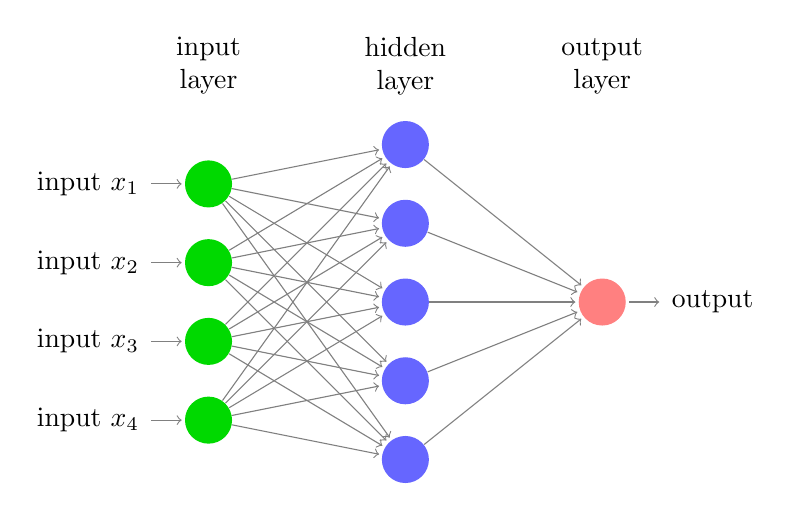
\begin{tikzpicture}[shorten >=1pt,->,draw=black!50, node distance=\layersep]
    \tikzstyle{every pin edge}=[<-,shorten <=1pt]
    \tikzstyle{neuron}=[circle,fill=black!25,minimum size=17pt,inner sep=0pt]
    \tikzstyle{input neuron}=[neuron, fill=black!15!green];
    \tikzstyle{output neuron}=[neuron, fill=red!50];
    \tikzstyle{hidden neuron}=[neuron, fill=blue!60];
    \tikzstyle{annot} = [text width=4em, text centered]

    % Draw the input layer nodes
    \foreach \name / \y in {1,...,4}
    % This is the same as writing \foreach \name / \y in {1/1,2/2,3/3,4/4}
        \node[input neuron, pin=left:input {$x_\y$}] (I-\name) at (0,-\y) {};

    % Draw the hidden layer nodes
    \foreach \name / \y in {1,...,5}
        \path[yshift=0.5cm]
            node[hidden neuron] (H-\name) at (\layersep,-\y cm) {};

    % Draw the output layer node
    \node[output neuron,pin={[pin edge={->}]right:output}, right of=H-3] (O) {};

    % Connect every node in the input layer with every node in the
    % hidden layer.
    \foreach \source in {1,...,4}
        \foreach \dest in {1,...,5}
            \path (I-\source) edge (H-\dest);

    % Connect every node in the hidden layer with the output layer
    \foreach \source in {1,...,5}
        \path (H-\source) edge (O);

    % Annotate the layers
    \node[annot,above of=H-1, node distance=1cm] (hl) {hidden layer};
    \node[annot,left of=hl] {input layer};
    \node[annot,right of=hl] {output layer};
\end{tikzpicture}
% feedforward network??
\caption[Example structure Neural Network]{Example structure of a fully connected NN: Every circle denotes one neuron. This example network consists of three layers. The weights of the connections between the neurons are omitted in this figure.}
% reference somehow to http://www.texample.net/tikz/examples/neural-network/ where it's taken from.}
\label{draw:neural_network}
\end{figure}

One neuron consists of several \emph{inputs}~$x_i$, an \emph{activation function} $\alpha$ that processes these inputs, and one \emph{output~o}. % (see equation~\ref{eq:output_neuron}).

\begin{equation}
o = \alpha \left(\sum_{i=1}^n x_i \cdot w_i + b_k\right)
\label{eq:output_neuron}
\end{equation}

Every input value of a neuron is scaled by its corresponding \emph{weight} $w_i$.
The \emph{bias} $b_k$ influences the behaviour of the neuron by increasing or decreasing the sum of the scaled input values for the calculation of the output of the neuron.
The number of summands $n$ denotes the number of input values of the neuron.
%This output is defined by the so called activation function  that takes the input values scaled by the corresponding weights, and the bias value as parameters. The number of summands $n$ is the number of inputs of the neuron.

The specific output of the neuron depends on the kind of activation function $\alpha$:
Common activation functions are the sigmoid function (equation~\ref{eq:sigmoid_simple}) and the rectified linear unit (ReLU) (equation~\ref{eq:rectifier_fct}). The input of the activation function $\left( \sum_{i=1}^n x_i \cdot w_i + b_k\right)$ is abbreviated as $z$. % check if mathematically correct
% citations for equations needed
% maybe: insert graph of sigmoid, rectifier graph

\begin{equation}
\label{eq:sigmoid_simple}
sigmoid(z) = \frac{1}{1 + e^{-z}} = \frac{e^z}{e^z + 1}
\end{equation}

\begin{equation}
\label{eq:rectifier_fct}
rec(z) = z^+ = \max(0, z)
\end{equation}

For an example neuron structure with more detailed description see figure~\ref{draw:neuron}.

As the NN consists of many neurons, it consists also of the corresponding weights $w_i $ and biases $b_k$. The weights and biases are also referred to as \emph{parameters}.
The neurons of a NN are arranged into \emph{layers}.
These layers are distinguished into one input layer, hidden layers and one output layer.
In the network example in figure \ref{draw:neural_network}, the green layer is referred to as input layer, the red layer as output layer. The layers in between input and output layer, in the example one blue layer, are referred to as hidden layers. 
The network example is a \emph{Fully Connected Network (FCN)}: The output of each neuron in one layer is connected to each neuron in the following layer~\cite{long2015_FCNs}.

In this work, the calculation of the final output of the network with respect to its current weights and biases is denoted as $y_{w,b}(x)$. $x$ contains the input values to the network and can for example have vector or matrix shape.
% besser erklären: y "enthält" weights und biases?


% maybe citation unnecessary
% also abbreviate singular: NN, denote "network" as abbreviation of NN?

% maybe put weights more beautiful on arrow
% uncommented this because IT'S SO SLOW DURING COMPILATION
\begin{figure}
\centering
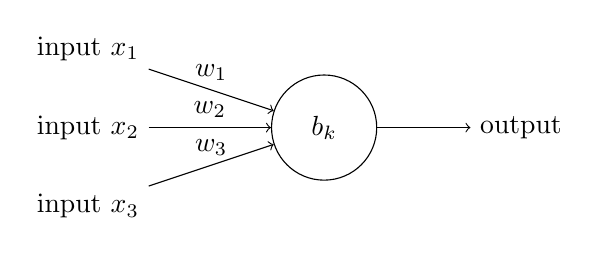
\begin{tikzpicture}
\path (0, 0) node[circle, draw, minimum size=38pt] (neuron) {$b_k$};
\path (-3, -1) node (arrow1start) {input $x_3$};
\path (-3, 0) node (arrow2start) {input $x_2$};
\path (-3, 1) node (arrow3start) {input $x_1$};
\path (2.5, 0) node (arrowfinalstart) {output};
\draw[->] (arrow1start) -- node[above] {$w_3$} (neuron);
\draw[->] (arrow2start) -- node[above] {$w_2$} (neuron);
\draw[->] (arrow3start) -- node[above] {$w_1$}(neuron);
\draw[->] (neuron) -- (arrowfinalstart);
\end{tikzpicture}
\caption[Example structure neuron]{General structure of a \emph{neuron}: The input values of the neuron are $x_1, x_2, x_3$. These input values are scaled by their corresponding weights $w_1, w_2, w_3$. $b_k$ denotes the bias. 
In this example, the output of the neuron using the sigmoid activation function is calculated by~$o={sigmoid\left(\sum_{i=1}^3 x_i \cdot w_i + b\right)}$.}
\label{draw:neuron}
\end{figure}

\subsection{Training Data}
\label{nn:training_data}
%The proposed training method in this work belongs to the \emph{supervised} learning methods, because the desired output of the network is known during the training process % When training a NN with data where the corresponding ground truth is unknown, the training procedure belongs to the \emph{unsupervised} learning methods. -> zu ausführlich, unsupervised weglassen
\emph{Training data} is used for the training process (see section~\ref{nn:training_methods}) of a NN. This training data is often composed of several datasets, later referred to as \emph{training sets}. One training set $\{(x_1,t_1),...,(x_j,t_j),...,(x_N,t_N)\}$ contains $N$ \emph{training samples} $(x_j,t_j)$ with one \emph{training input}~$x_j$ and the corresponding \emph{target $t_j$}.

The input given to the NN is denoted as $x_j$. The desired output of the network for the corresponding $x_j$ is $t_j$. The target $t_j$ is also referred to as \emph{ground truth} or \emph{label}. 
Since for each input $x_j$ the corresponding ground truth $t_j$ is known, this is referred to as a \emph{supervised} machine learning problem.

When there is little training data available, the network can not be trained sufficiently to predict the desired output. % insert citation here
The approach to train the network for many iterations with the same, small training dataset can cause overfitting (see section~\ref{nn:testing}).
To avoid this problem, a commonly used method is \emph{data augmentation}: The dataset is artificially enlarged by operations on the different training samples $(x_j,t_j)$. Commonly used transformations are, given that the input of the network are images, translation~\cite{augmentation_SAR2016Ding}, horizontal and vertical reflections, and altering the RGB channels of the images.~\cite{imageNetWinner2012krizhevsky}

\subsection{Network Training}
\label{nn:training_methods} % maybe another heading  
The general aim of training a NN is that, after the training is finished, the network recognizes certain features of the input data and classifies the input accordingly. These features are learned by each weight $w_i$ and each bias $b_k$ of the network during the training phase.
% With this information learned during training, the NN is capable of predicting several \emph{classes} out of the given input. These classes are specified in the ground truth of the training set. ---> weglassen weil sonst classification problem erklären 
The resulting network out of a network structure that learned specific parameters is referred to as \emph{model}. 

The prediction result of a NN with given input $x$ is calculated as $y_{w,b}(x)$.
During the training period, the deviation between $y_{w,b}(x_j)$ for the training input $x_j$ and the corresponding desired output $t_j$ is calculated and referred to as error $E_j$.
The aim is to adjust the parameters of the network in a way that $E_j$ is minimized.

% loss function: decides how to calculate the difference between output and desired output
The \emph{loss function} $L(y_{w,b}(x_j), t_j)$ of the NN specifies the way how $E_j$ is determined for one training sample $(x_j,t_j)$.
The loss function is also often referred to as cost function. 
% The function $y_{w,b}(x_j)$ calculates the output of the network respective to its current weights and biases, given the input $x$. -> maybe to much detail

One of the most common loss functions is the mean squared error (MSE):
\begin{equation}
MSE(y_{w,b}(x_j), t_j) = (t_j-y_{w,b}(x_j))^2
\label{eq:mean_sq_error}
\end{equation}

As the loss $L(x_j,t_j)$ is calculated for each training sample , the results are summed and then averaged over the complete training set $\{(x_1,t_1),...,(x_j,t_j),...,(x_N,t_N)\}$. This calculation of the overall error $E$ is stated in equation~\ref{eq:mean_loss_all_inputs} for $N$ training inputs.

\begin{equation}
E = \frac{1}{N} \sum_{j=1}^N L(y_{w,b}(x_j), t_j)
\label{eq:mean_loss_all_inputs}
\end{equation}

$E$ is reduced by adjusting the weights and biases of the network with the \emph{gradient descent} method~\cite{backprop_grad_desc_closed1993shun}. 
To reduce $E$, the partial derivatives of the loss function with respect to all $G$ weights $w_i$ and all $D$ biases $b_k$ of the network are calculated stepwise.
Afterwards, each weight $w_i$ and each bias $b_k$ in $y_{w,b}(x_j)$ is adjusted.
%The loss function is derivated partially by weights and biases that are part of the parameter $y_{w,b}(x_j)$. 
The partial derivatives are contained in two \emph{gradients} of the loss function: $\nabla E_{w}$ for the weights and $\nabla E_{b}$ for the biases of the network.

\begin{equation}
\nabla E_{w} = \left(\frac{\partial E}{\partial w_1} , ... ,\frac{\partial E}{\partial w_i}, ... , \frac{\partial E}{\partial w_G}\right)^T
\label{eq:gradient_weights}
\end{equation}

\begin{equation}
\nabla E_{b} = \left(\frac{\partial E}{\partial b_1} , ... , \frac{\partial E}{\partial b_k}, ... , \frac{\partial E}{\partial b_D}\right)^T
\label{eq:gradient_biases}
\end{equation}

Every weight $w_i$ and every bias $b_k$ in the loss function is updated to $w'_i$ and $b'_k$ by using the entries of $\nabla E_{w}$ and $\nabla E_{b}$.

\begin{equation}
w'_i = w_i - \lambda \frac{\partial E}{\partial w_i} 
\label{eq:update_weight} 
\end{equation}

\begin{equation}
b'_k = b_k - \lambda \frac{\partial E}{\partial b_k}  
\label{eq:update_bias}
\end{equation}

The parameter $\lambda$ refers to the \emph{learning rate}. It is used to control the learning process of the network by scaling the adjustment of the weights and biases. % citation needed -> include general book that explains this at beginning
% maybe include word "update rule"

The gradients $\nabla E_{w}$ with $G$ entries and $\nabla E_{b}$ with $D$ entries are summarized into one gradient $\nabla E$. 

\begin{equation}
\nabla E = \left(\frac{\partial E}{\partial w_1},..., \frac{\partial E}{\partial w_i}, ... ,\frac{\partial E}{\partial w_G},\frac{\partial E}{\partial b_1}, ..., \frac{\partial E}{\partial b_k}, ..., \frac{\partial E}{\partial b_D}\right)^T
\label{eq:nabla_L}
\end{equation}

Each entry $\frac{\partial E}{\partial w_i}$ and $\frac{\partial E}{\partial b_k}$ of $\nabla E$ is calculated separately for every training sample $(x_j,t_j)$, and then averaged over all $N$ training samples.

\begin{equation}
\nabla E = \frac{1}{N} \sum_{j=1}^{N} \nabla E_j
\label{eq:mean_nabla_L}
\end{equation}

Calculating the gradient over all the training samples and afterwards averaging the result is computationally expensive. 
To reduce the learning time of the network, it is common to use a modified gradient descent method: It is denoted as \emph{stochastic gradient descent}. % maybe cite here  
The gradient $\nabla E$ is estimated by calculating the gradient for a subset of $\beta$ samples out of the training set, and then averaging the result: $\frac{1}{\beta} \sum_{i=1}^\beta \nabla E_i$.
The subset of the original training set is referred to as \emph{mini-batch}. The number of elements of the mini-batch, $\beta$, is the \emph{batch size}. Training the NN with randomly picked mini-batches also has the advantage of avoiding shifts of the network.~\cite{batch_normaliz2015ioffe}
When the complete training dataset was shown to the network, i.e. every element of the training dataset was propagated through the network one time, one \emph{epoch} of training is completed.

% not sure if this backprop description is correct:
\emph{Backpropagation~(BP)}~\cite{rumelhart1986origin_backprop_paper} is one way to efficiently calculate all partial derivatives of the network~\cite{backprop_grad_desc_closed1993shun}.
It is by far the most common approach for training NNs~\cite{hernandez_adams2015prob_backprop}.
First, the forward pass of the training phase is performed: The output of the NN is calculated out of the given input.
The gradients $\nabla E_j$ are calculated for each input of the mini-batch by backpropagating the error $E_j=L(y_{w,b}(x_j), t_j)$ back through the network. Then, the update step is performed: Every weight $w_i$ and bias $b_k$ of the network is corrected according to the calculated gradients.~\cite{rumelhart1986origin_backprop_paper}~\cite{buscema1998backprop_network}  

\subsection{Network Testing}
\label{nn:testing}

%% generalization error 
When training a NN, the aim is to obtain a network with optimal generalization performance. Generalization performance means that $E$ is minimal on network inputs not seen during training. This $E$ is also referred to as \emph{generalization error}.~\cite{cross_val_overfit1998prechelt}

Therefore, when testing the performance of a NN, it is necessary to provide input that was not given to the network during the training procedure. These previously unseen input data is referred to as \emph{test data}.
This test data is composed of several \emph{test sets}. One test set $\{(\mathbf{x_1},\mathbf{t_1}),...,(\mathbf{x_l},\mathbf{t_l}),...,(\mathbf{x_M},\mathbf{t_M})\}$ consists of $M$ \emph{test samples} $(\mathbf{x_l},\mathbf{t_l})$ with one test input $\mathbf{x_l}$ and its corresponding target $\mathbf{t_l}$.

When the generalization error increases during training, this indicates a problem that is denoted as \emph{overfitting}: While the network seems to get better and better during training, i.e. $E$ on the training dataset decreases, the network actually begins to predict worse on the test set, the generalization error increases.~\cite{cross_val_overfit1998prechelt}
The prediction performance of the network is fitted to the training dataset, but generalizes poorly.

It is a commonly used method to split the given data into separated training and testing sets and evaluate the network with the \emph{cross-validation} method. 

In \emph{k-fold cross-validation}, all training data is assigned randomly to $k$ datasets with approximately the same size. These $k$ datasets are separated into $k-1$ training sets and in one remaining test set. 
The NN is trained on the $k-1$ training sets and then evaluated on the remaining test set. This procedure is done $k$ times. Each time another set is chosen as test set, consequently the training sets are also different each time. As a result, there are $k$ different models of the NN. The performance of the NN is evaluated by testing each model on its corresponding test set and averaging the results over all models.

Another variant of k-fold cross-validation is \emph{leave-one-out cross-validation (LOOCV)}: 
For the given training data with $N$ elements, one sample $(\mathbf{x_l},\mathbf{t_l})$ is chosen as test sample, the rest of the data as training samples. Every element is chosen once as a test sample. The performance of the resulting models is evaluated the same way as for k-fold cross-validation, with $k=N$.

Cross-validation is a useful method to estimate the generalization error: The evaluation of the network includes all available labeled data without having used it for training and testing at the same time.~\cite{loocv_prev_overfit1997Ng} 

%%% pre-trained 
A NN structure which has already adjusted weights and biases due to previous training on several datasets, for example ImageNet~\cite{pre_trained_overfit2016marmanis}, is also referred to as \emph{pre-trained} network.
%When solving tasks like for example image recognition by using pre-trained networks, $E$ is reduced in comparison to using randomly initialized networks for the task~\cite{imageNetWinner2012krizhevsky}.
%The problem of overfitting is reduced by using a pre-trained network, especially when there are few training data available.~\cite{pre_trained_overfit2016marmanis} -> correction to:
Using pre-trained networks instead of randomly initialized networks to solve tasks such as image recognition reduces both $E$
and overfitting, especially when there are few training examples available\cite{imageNetWinner2012krizhevsky, pre_trained_overfit2016marmanis}.

\section{Convolutional Neural Network}
\label{cnn:general}
A \emph{Convolutional Neural Network (CNN)} is a specific kind of NN. The first application of CNNs was developed by LeCun et al.~\cite{first_cnn1998lecun}. In the following, the structure of a CNN is explained, given that it is used for image recognition.

% input image == values of first "feature map"
% Input of a CNN: Matrix with three dimensions -> 2 dimensions are image resolution 
In this scenario, the input to a CNN consists of an image with three dimensions. For example a RGB image has two dimensions for the resolution and one dimension for the RGB channels. This input is referred to as \emph{input layer}, the dimensions as \emph{channels}.

%One layer consists of several \emph{feature maps} (?)
% "spatial dimensions": first 2 dimensions / height, width
One CNN consists of multiple \emph{feature maps}, see for example U-Net in figure~\ref{img:basic_u-net}.
These feature maps usually have three dimensions: Two spatial dimensions for width and height, and a third dimension which denotes the number of channels. The input image is also a feature map.

Convolutions with a specific kernel size are applied to the feature maps, followed by an activation function $\alpha$ (see section~\ref{nn:general}). The result of the convolutions is stored in the following feature map of the CNN. The kernel is also referred to as \emph{filter}.
In a CNN structure, the parameters of the neurons are not realized with direct connections between neurons like in a general NN: They are stored in the filters of the CNN.
The learning process with gradient descent works like for NNs in general, but in particular the weights of the filters of the CNN are updated.

The number of feature map dimensions and filter dimensions is always the same.
The first two dimensions of the filter are applied to the spatial dimensions of the feature map. These dimensions of the filter are usually smaller than the corresponding feature map dimensions it is applied to. 
% The width and height of the kernel are smaller than the feature map is is applied to.
The third dimension of the filter always has the same size as the number of channels of its input feature map. This means that the filter extends through the full depth of its input volume.~\cite{lecun1990handwritten_digit_recog} 
The \emph{stride} of a filter denotes the distance between the regions of the feature map it is applied to.

The state-of-the-art CNNs, especially for image segmentation, consist of one \emph{downsampling phase} followed by an \emph{upsampling phase}. These are also denoted as \emph{encoder} and \emph{decoder} of the network.
In the downsampling phase, the input of the network is reduced stepwise by convolutions. % at the same time the number of feature maps is increased. 
In the upsampling phase, the size of the output after the downsampling phase is increased again by application of deconvolutions.~\cite{Shvets2018, du2018_2D_pose_est_CNN} 
U-Net~(see figure~\ref{img:basic_u-net}) proposed by Ronneberger et al.~\cite{Ronneberger2015} is a typical encoder-decoder CNN used for segmentation of images (see figure~\ref{img:basic_u-net}). 

\begin{figure}
	\centering
	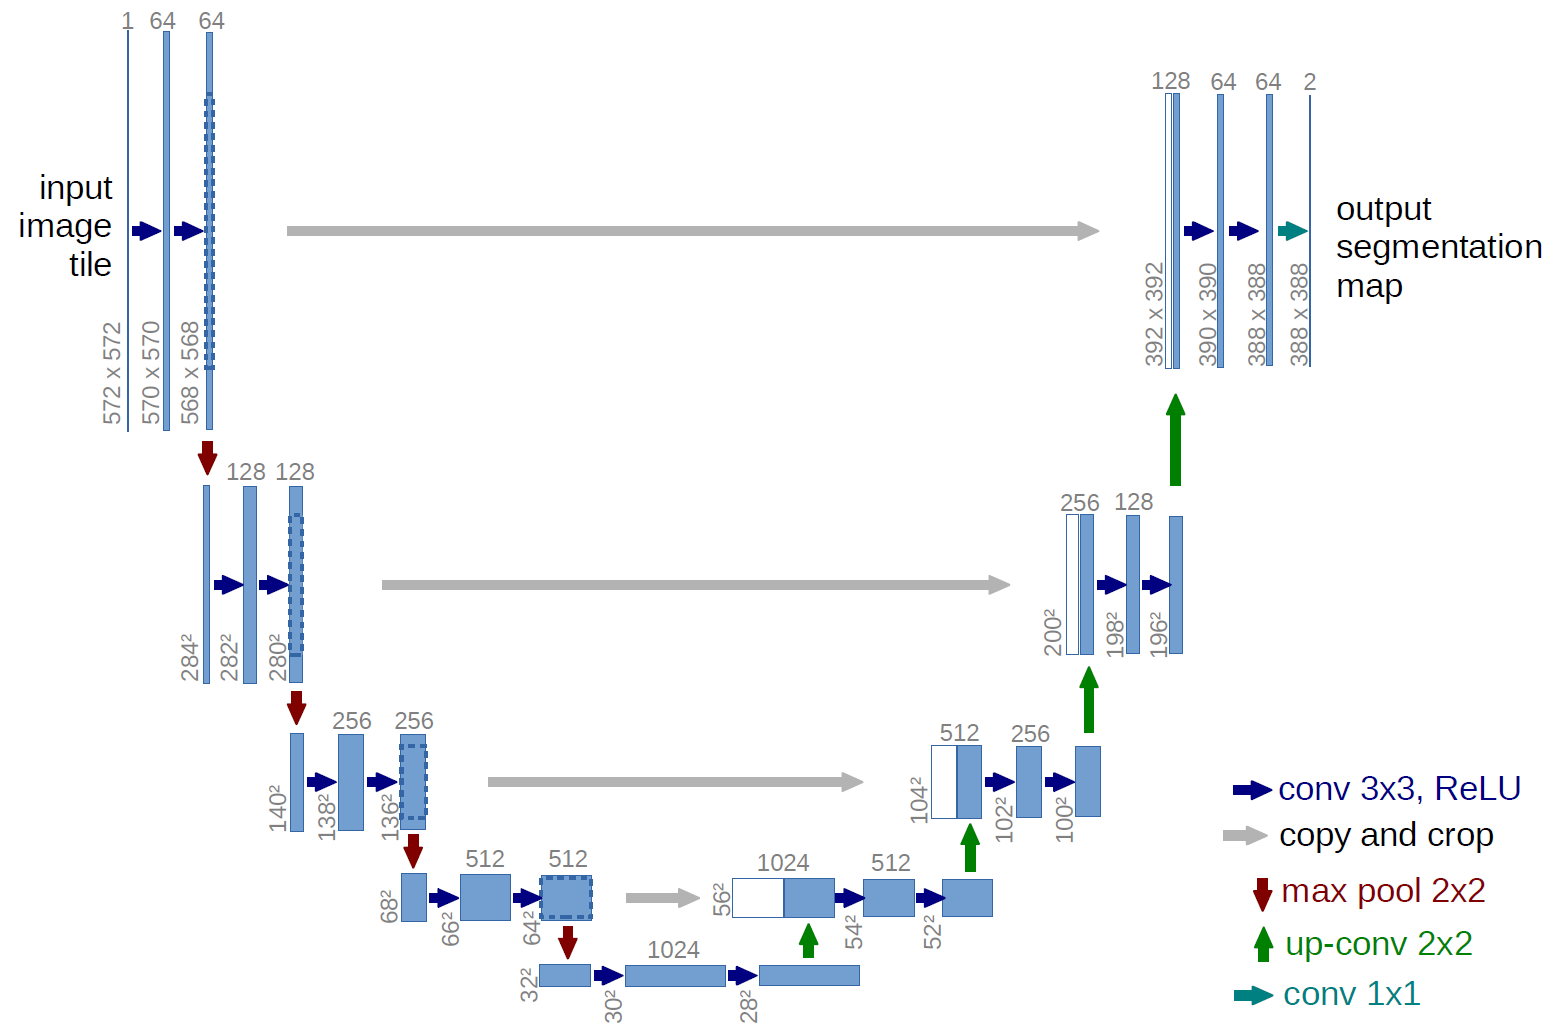
\includegraphics[width=.7\textwidth]{images/networks/u-net-architecture.png}
	\caption[Structure of U-Net]{Structure of U-Net, proposed by Ronneberger et al.~\cite{Ronneberger2015}. Each blue box corresponds to a multi-channel feature map. The number of channels is denoted on top, the resolution of the map is denoted at the left side of the box. White boxes refer to feature maps that are copied from the encoder phase and concatenated to the decoder phase. The arrows denote the operation types of the network.}
	\label{img:basic_u-net}
\end{figure}

There exist different kinds of convolutions. In the encoder phase of the network, the applied convolutions mostly preserve or reduce the spatial dimensions of the input and increase the number of channels. 
In the decoder phase, the convolutions mostly preserve or increase the spatial dimensions of the input and decrease the number of channels. This type of convolution is referred to as \emph{transposed convolution}, \emph{deconvolution} or \emph{upconvolution}. To increase the spatial dimensions, \emph{padding} is included for the convolutions.
% give example pic for convolution / cite convolution

\emph{Pooling} in CNNs is realized by a filter that reduces the dimension of its input. It is a widely used method to downsample the feature maps in the encoder phase of the network. The most common pooling method is \emph{max pooling}: Only the maximum value of the input region of the filter is returned.

% optimizer

% explain RNN -> needs reference in State of the Art

% explain ex vivo (refer here from methods / explain in methods)
% explain morphology opening (refer here from methods / explain in methods)

%\subsection{Fully Convolutional Network} ->this is not really correct
%\label{sec:FCN}
% explain FCN -->Fully Convolutional Networks (FCN) are a particular type of CNN recently proposed by \cite{long2015_FCNs} out of \cite{garcia2017segm_nonrigid_book}, reference to "fully connected" explanation in NN -> isn't explained yet
%A widely used architecture for CNNs are Fully Convolutional Network (FCN). The basic operations like convolutions, pooling and activation functions operate on local receptive fields. In FCNs, these operations are applied completely to their input. The feature maps of a FCN are referred to as \emph{fully connected layers}.~\cite{long2015_FCNs}

